\section{Discussion of Gradient Checkpointing}
The below image provides a visual illustration of what the memory lifetime looks like with and without checkpointing. With rematerializing activations the blue curve shows that we use way lesser RAM than if we retain all activations as in the red curve. 
Gradient Checkpointing is also called rematerialization or recomputation. In practice, you can activate gradient recomputation in PyTorch using torch.utils.checkpoint API.

\begin{figure}[h]          % h=here, t=top, b=bottom, p=page
    \centering
    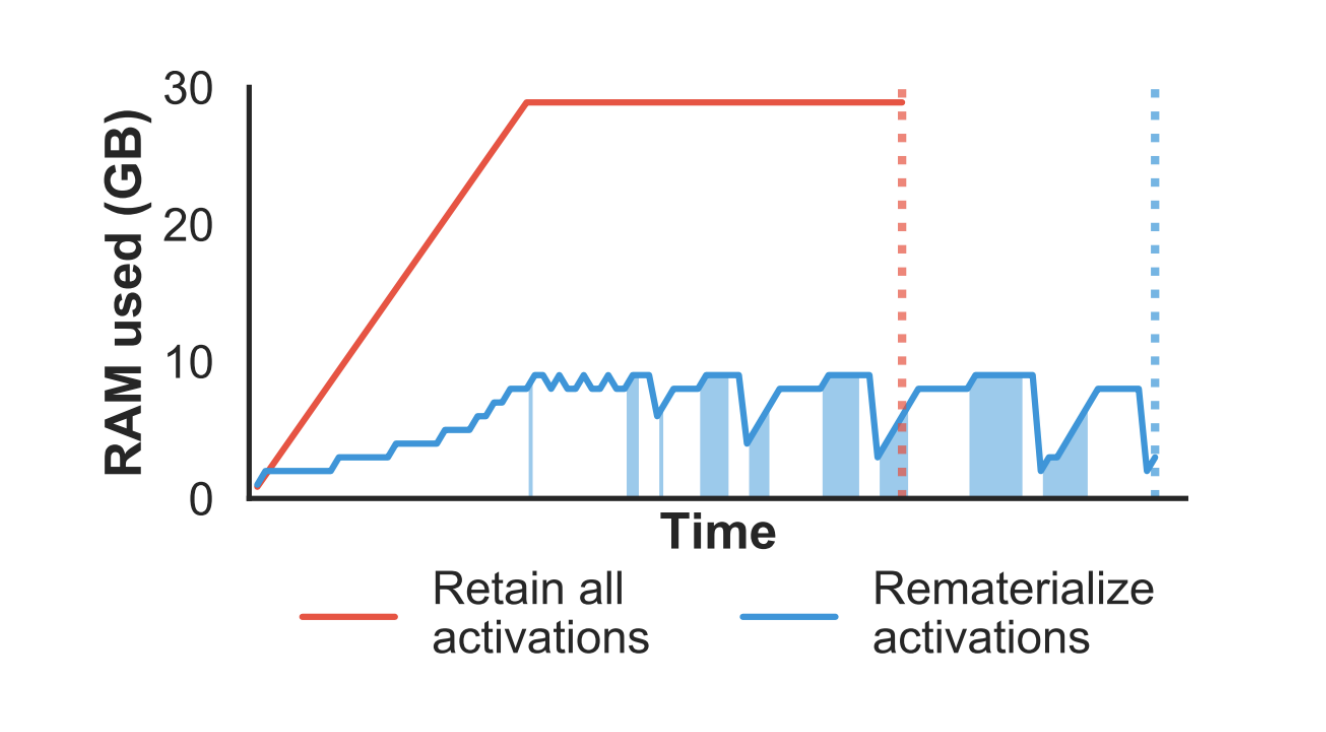
\includegraphics[width=0.8\textwidth]{memory_dynamics.png}
    \caption{Memory Dynamics}
    \label{fig:memory_dynamics}    % for cross-referencing
\end{figure}
Cons of this approach are that this only helps with the activation memory, not with weight or optimizer memory. If we have plenty of memory, we can retain all activations and we don't have to spend extra time recomputing them.

When thinking about the optimal checkpointing policy we need to consider things like the memory of the layers to be checkpointed (since different layer out's have different sizes) and the recomputation cost of the non-checkpointed layers since it won't be the same for all layers

\section{Similar approach: Gradient Accumulation}
Rematerialization wastes some compute by design. Gradient accumulation prevents that by keeping a small buffer of accumulated gradients. When the hardware can't fit your desired batch size, you run the training loop with smaller microbatches and accumulate the gradients into the buffer. We run iterations of microbatches and fill the buffer till desired batch size is reached and then run the gradient update.
However with this approach, in some cases when microbatches are too small, we risk having very low Arithmetic Intensity and poor GPU utilization. 